\chapter{Конструкторская часть}

В этом разделе будут приведены требования к вводу и программе, а также схемы алгоритмов нахождения расстояний Левенштейна и Дамерау-Левенштейна.

\section{Требования к вводу}
\begin{enumerate}
	\item На вход подаются две строки, которые могут быть пустыми.
	\item Буквы верхнего и нижнего регистров считаются различными.
\end{enumerate}

\section{Требования к программе}
\begin{enumerate}
	\item Обрабатывать корректно любые входные строки.
	\item В результате программа должна вывести число -- расстояние Левенштейна (Дамерау-Левенштейна).
	\item Возможность обработки строк, включающих буквы как на латинице, так и на кириллице.
	\item Наличие функциональности замера процессорного времени работы реализаций алгоритмов поиска расстояний Левенштейна и Дамерау-Левенштейна.
\end{enumerate}


\section{Разработка алгоритмов}

На вход алгоритмов подаются строки $S1$ и $S2$.

На рисунке \ref{fig:lev} представлена схема алгоритма поиска расстояния Левенштейна. На рисунках \ref{fig:DLrec} -- \ref{fig:DLiter} представлены схемы алгоритмов поиска расстояния Дамерау-Левенштейна.

\begin{figure}
	\centering
	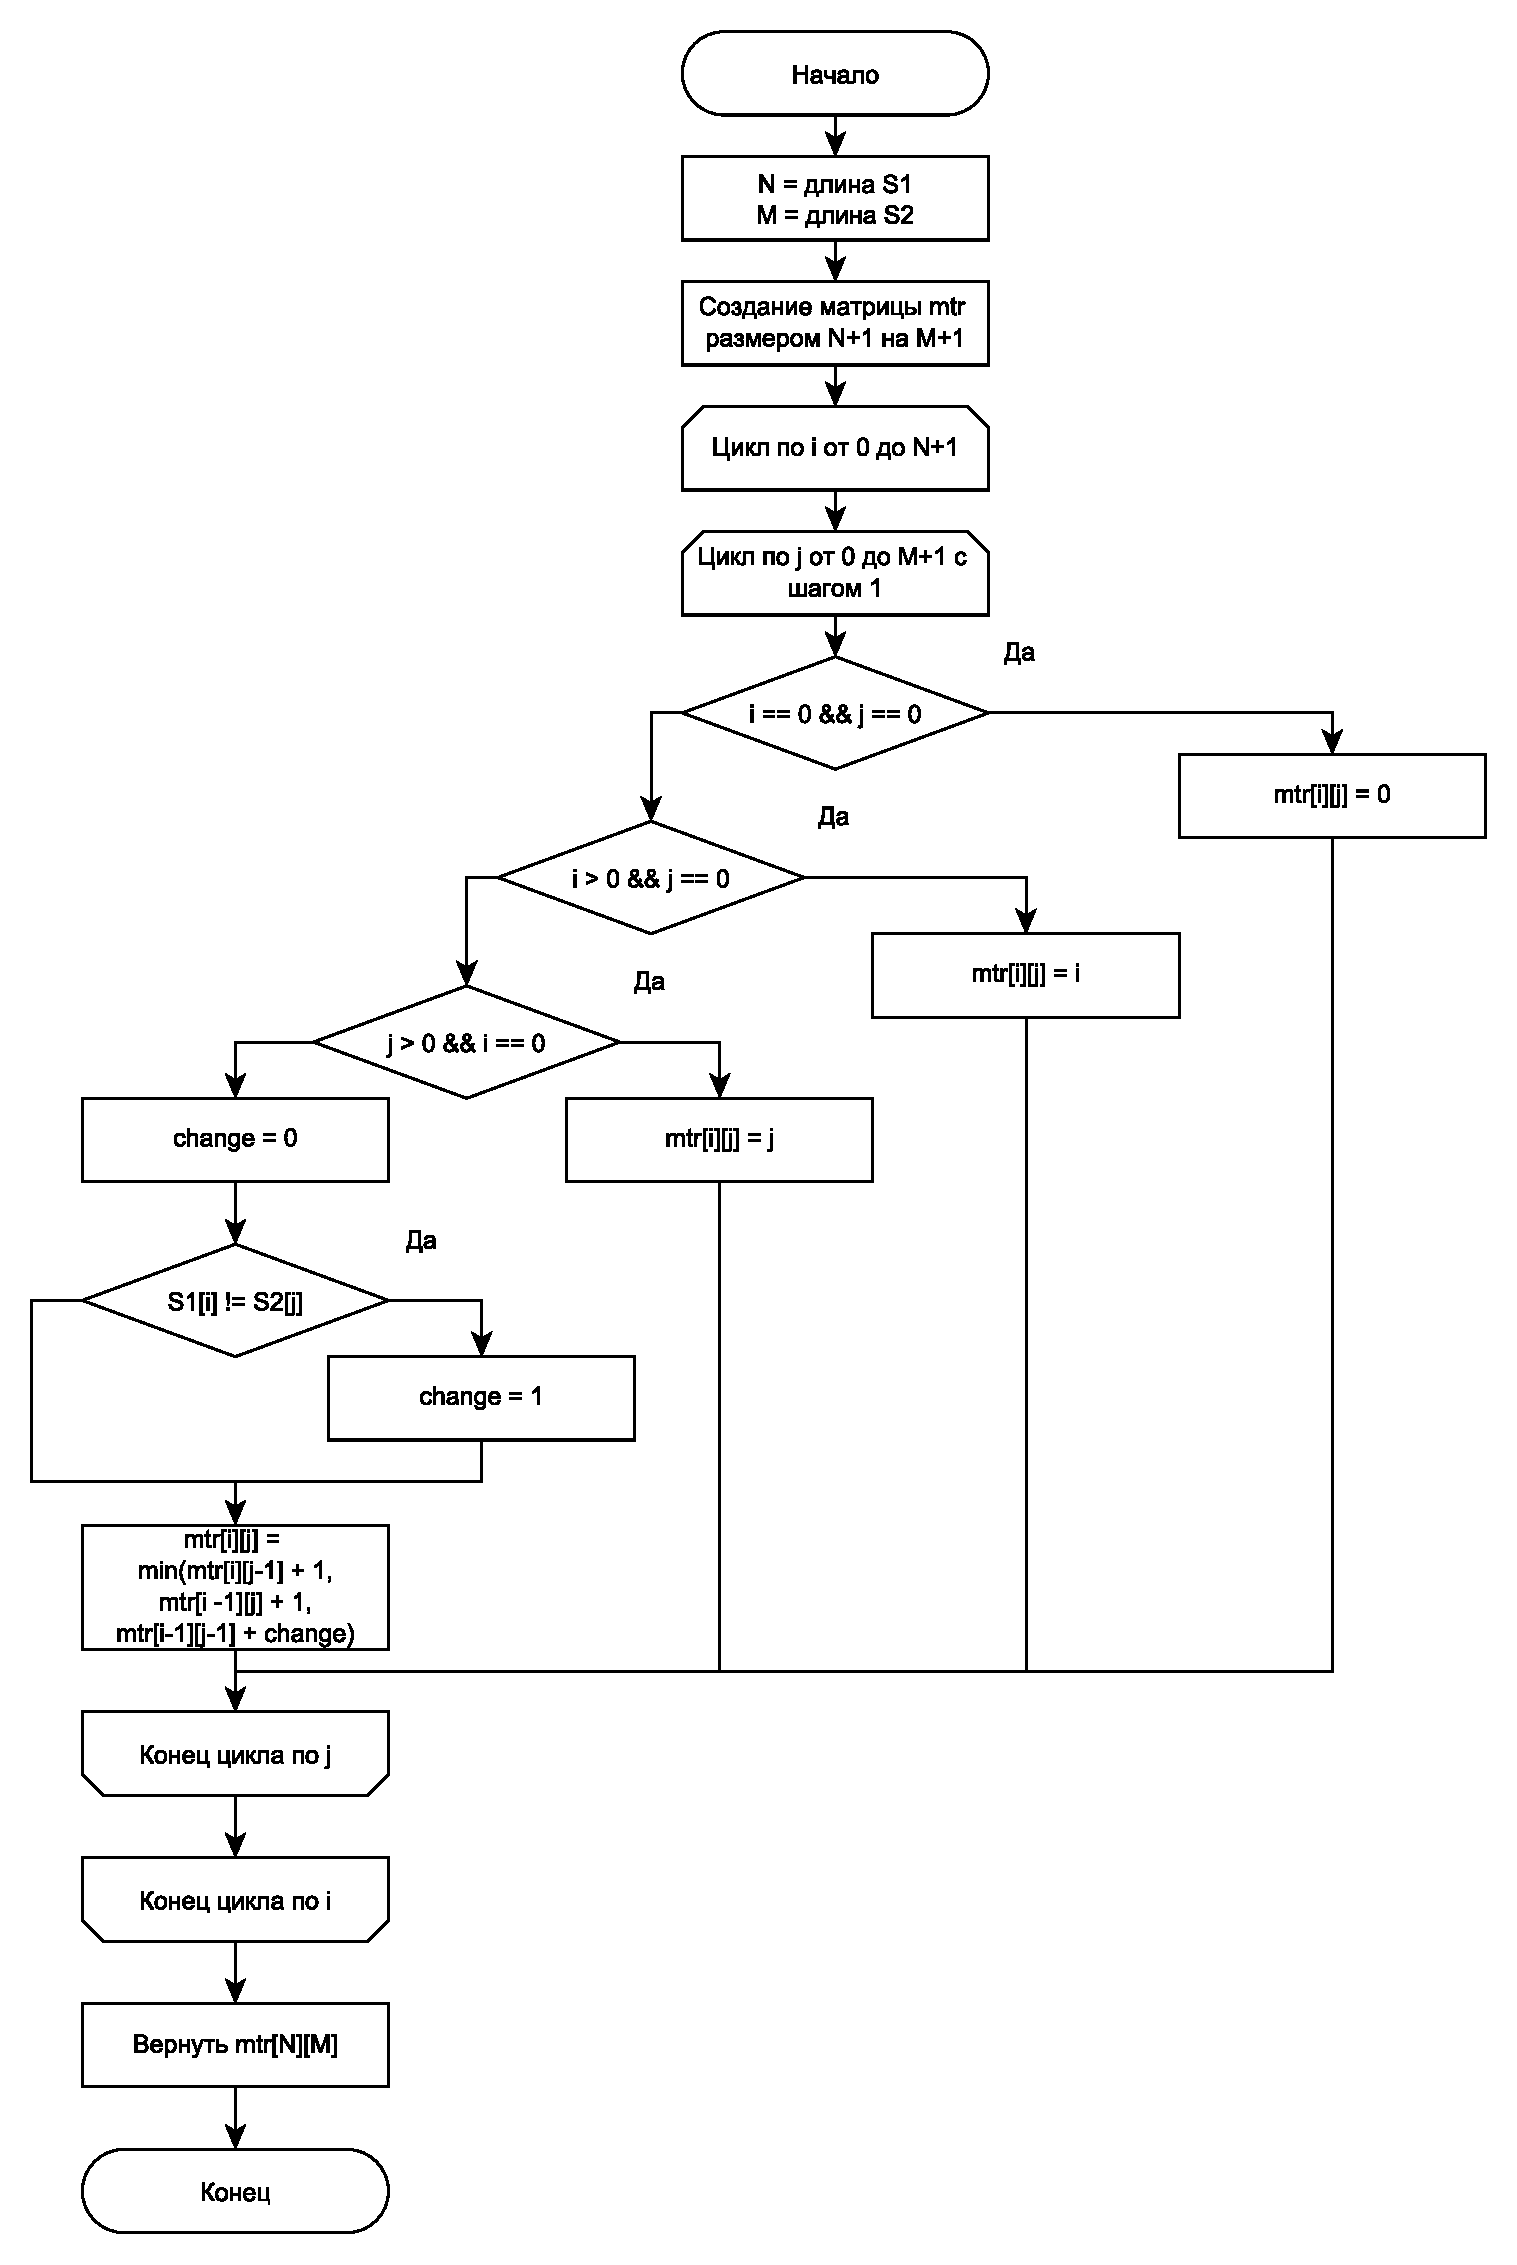
\includegraphics[width=0.9\textwidth]{img/lev2.pdf} % замените на имя вашего файла
	\caption{Нерекурсивный алгоритм нахождения расстояния Левенштейна}
	\label{fig:lev}
\end{figure}

\begin{figure}
	\centering
	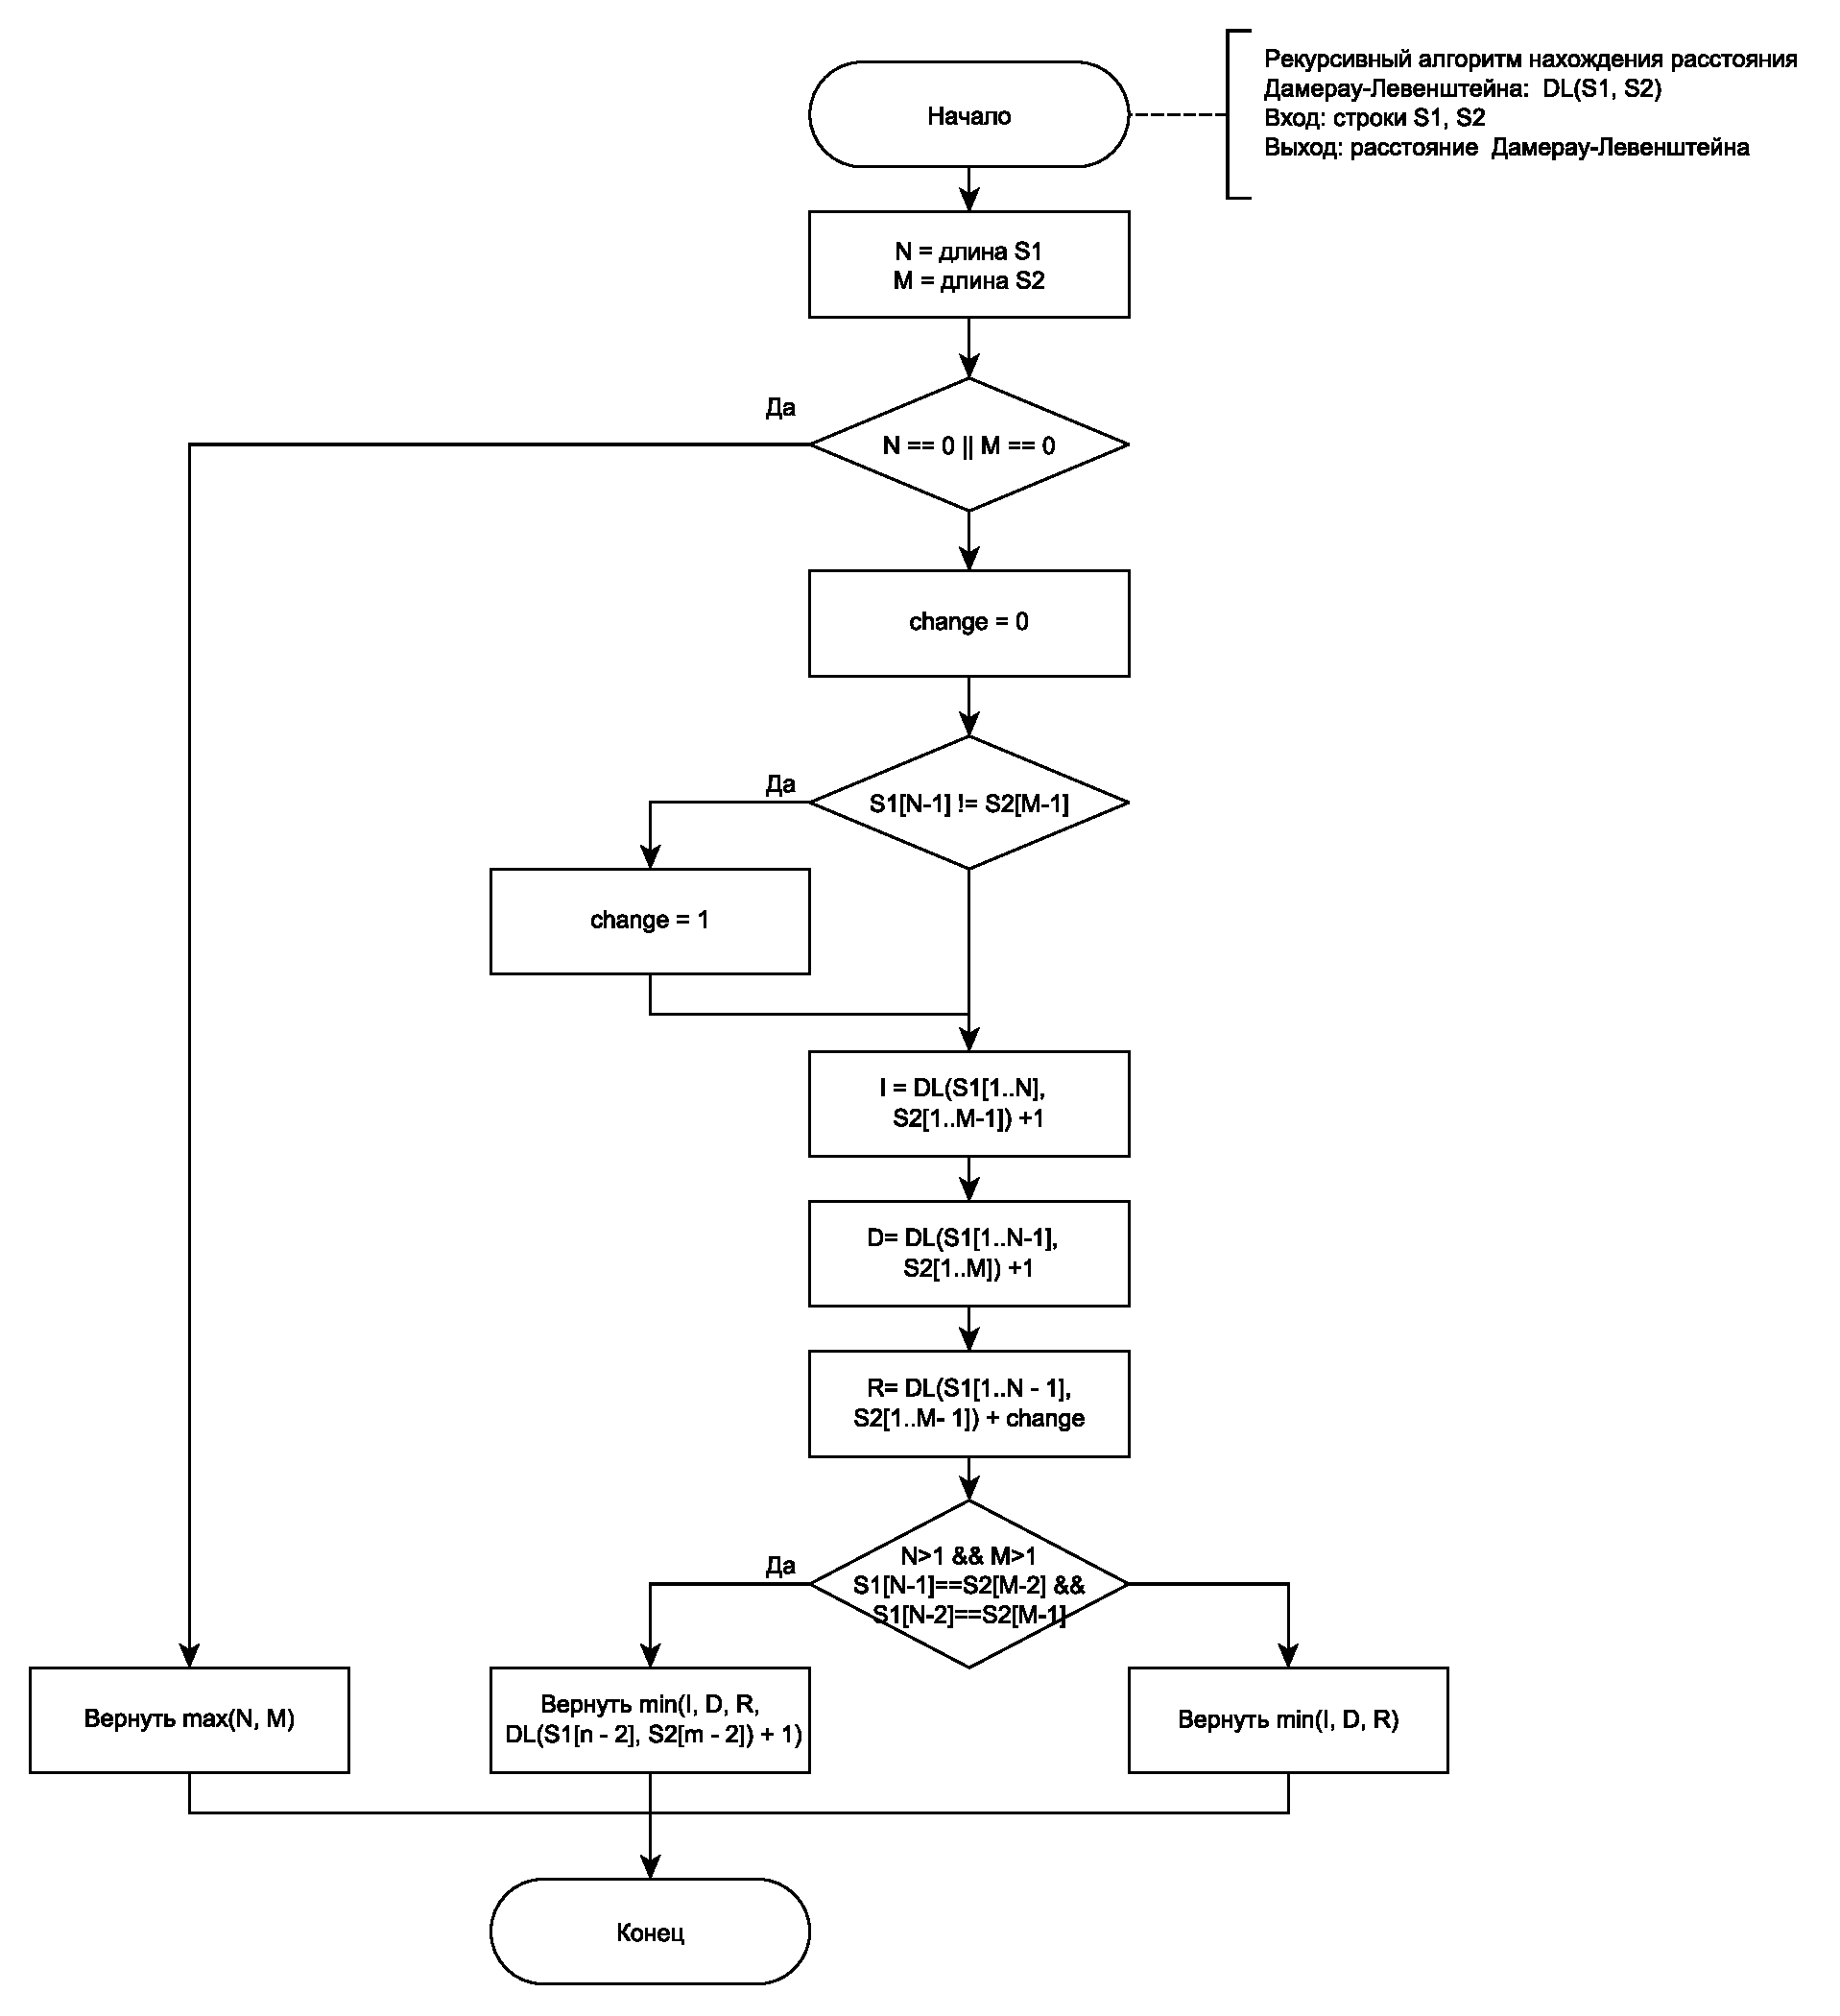
\includegraphics[width=1\textwidth]{img/DLrec.pdf} % замените на имя вашего файла
	\caption{Рекурсивный алгоритм нахождения расстояния Дамерау-Левенштейна}
	\label{fig:DLrec}
\end{figure}

\begin{figure}
	\centering
	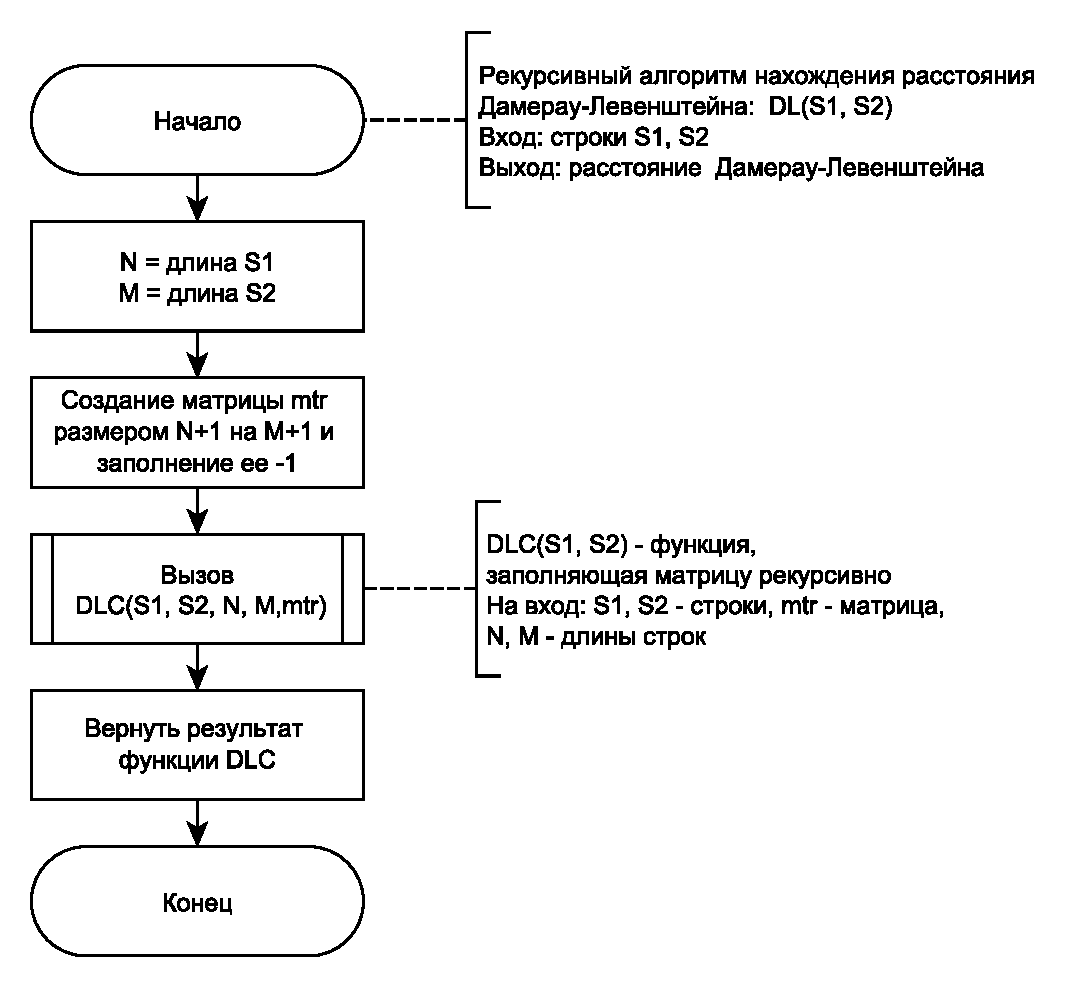
\includegraphics[width=1\textwidth]{img/DLrecCash.pdf} % замените на имя вашего файла
	\caption{Рекурсивный алгоритм нахождения расстояния Дамерау-Левенштейна с кешем}
	\label{fig:DLrecCash}
\end{figure}

\begin{figure}
	\centering
	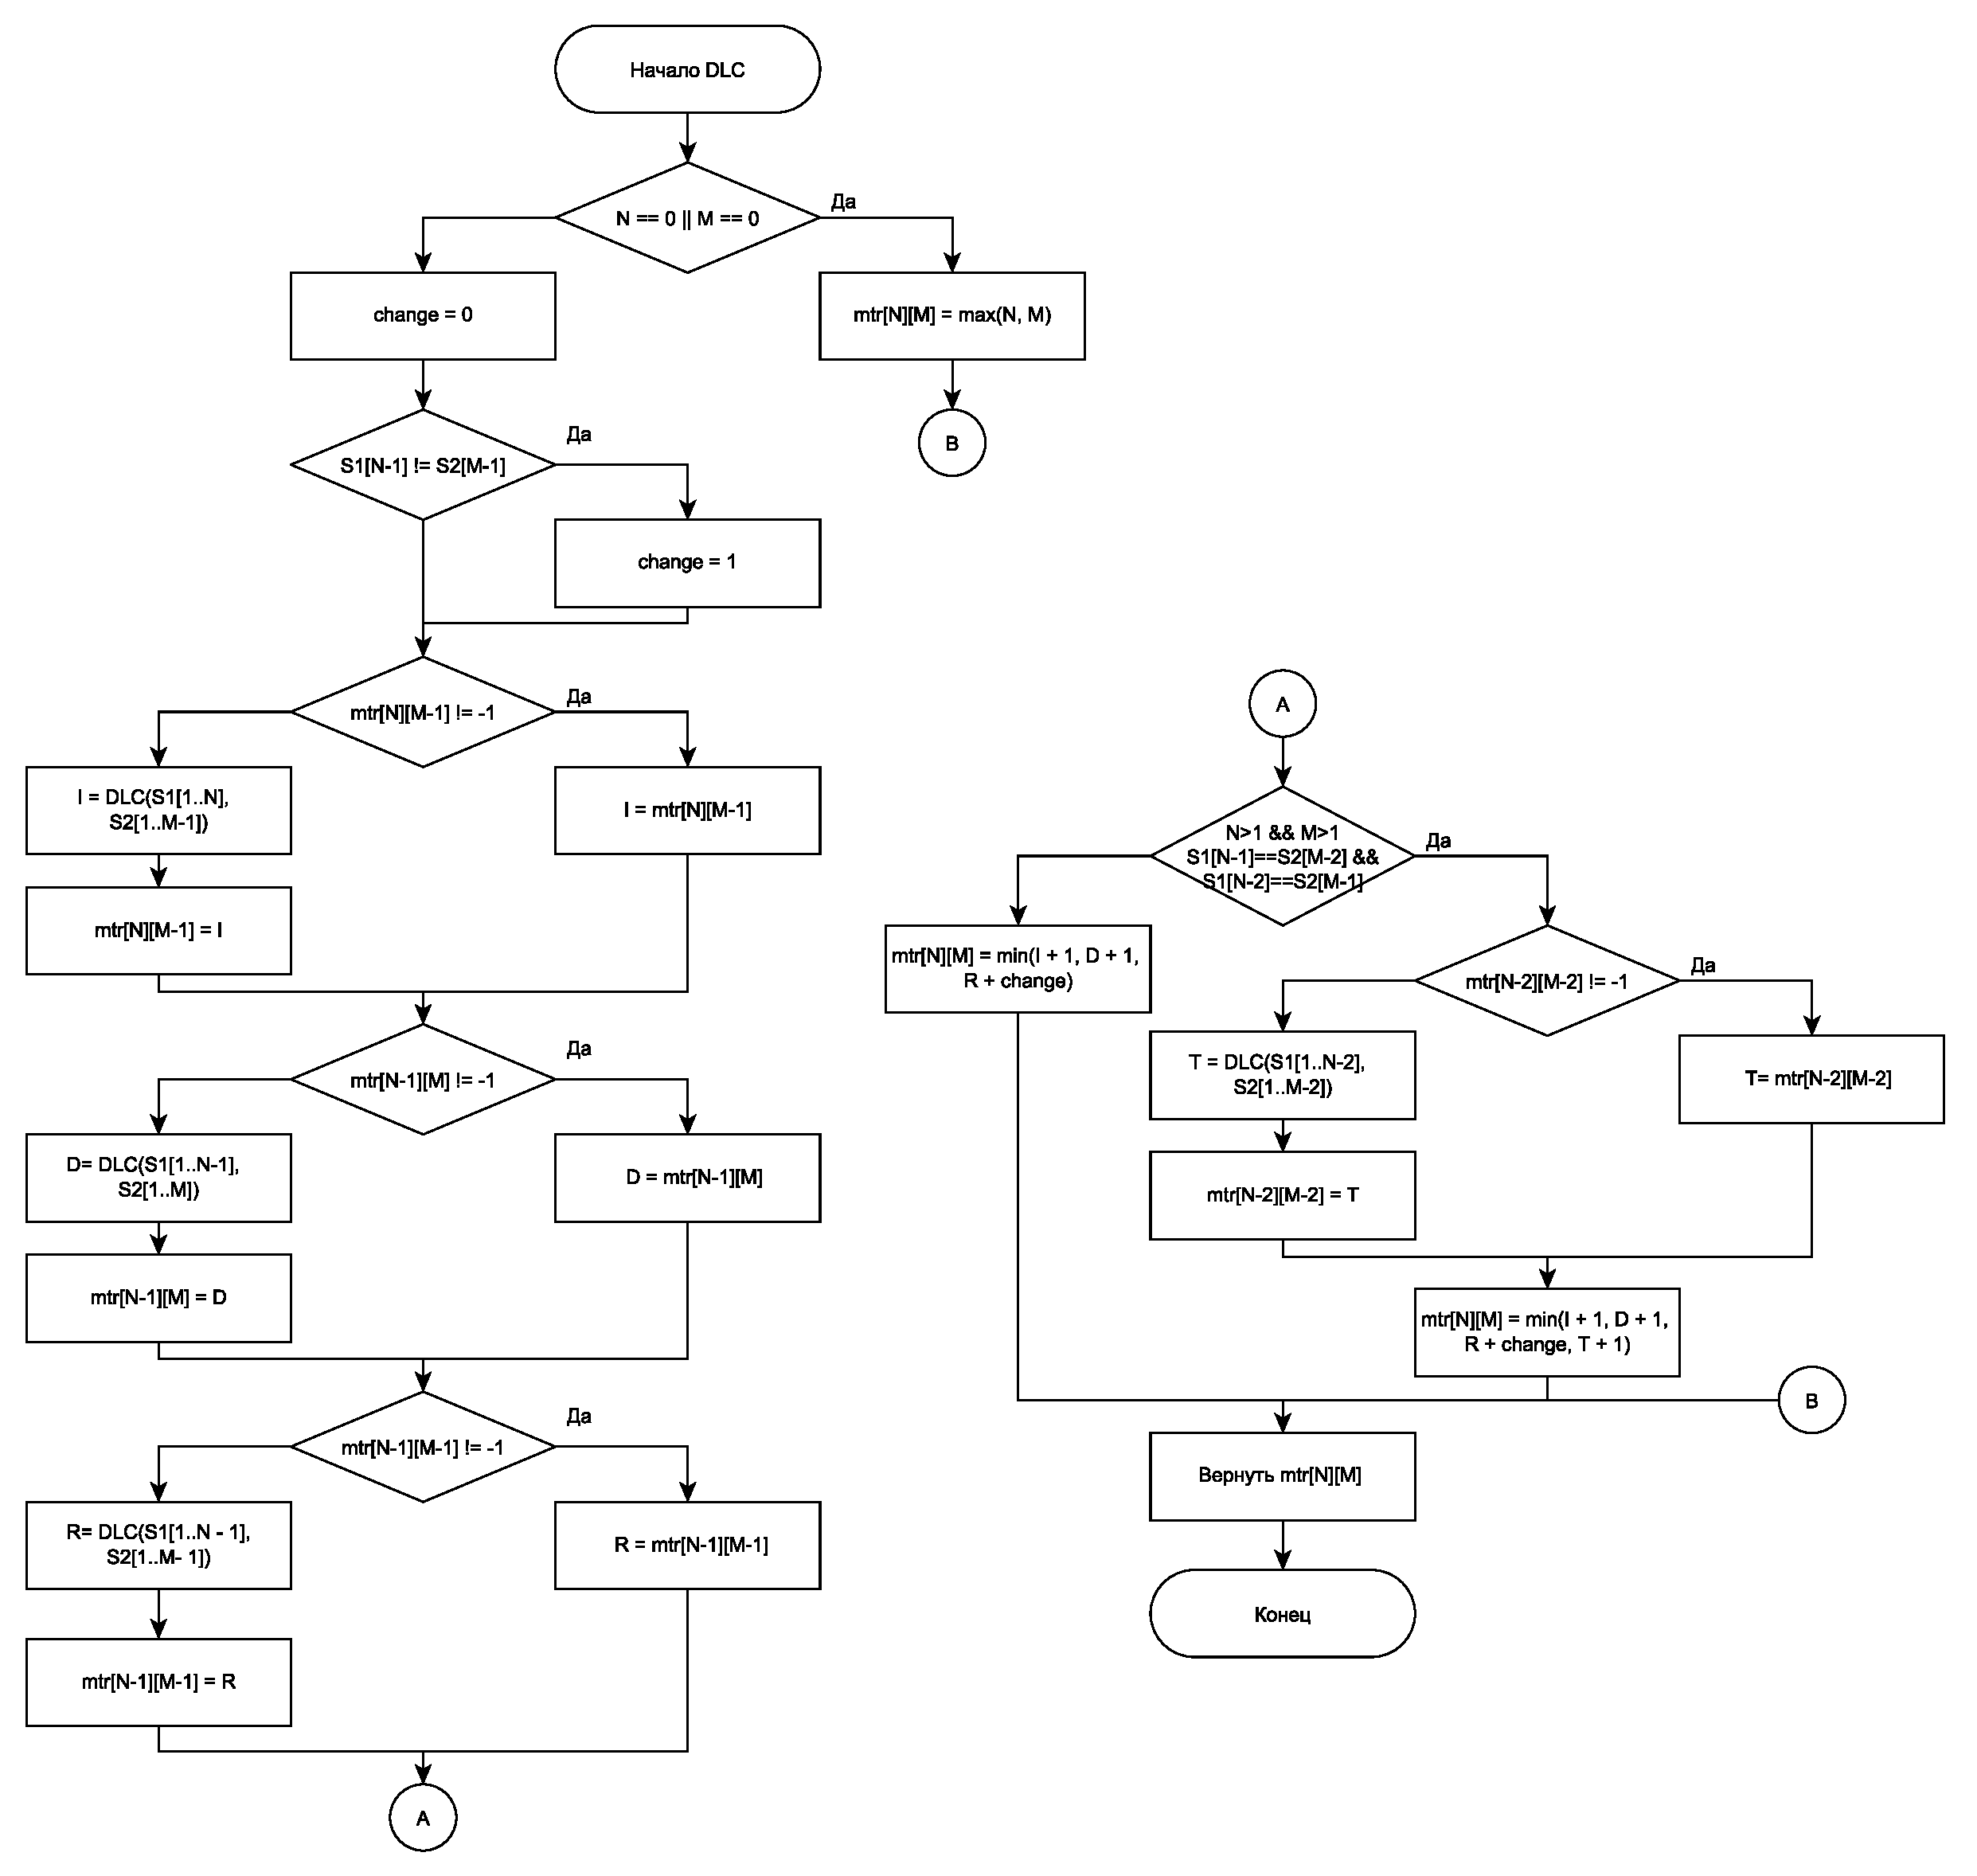
\includegraphics[width=1\textwidth]{img/DLrecCash2_1.pdf} % замените на имя вашего файла
	\caption{Функция заполняющая матрицу расстояний Дамерау-Левенштейна рекурсивно}
	\label{fig:DLrecCash2}
\end{figure}

\begin{figure}
	\centering
	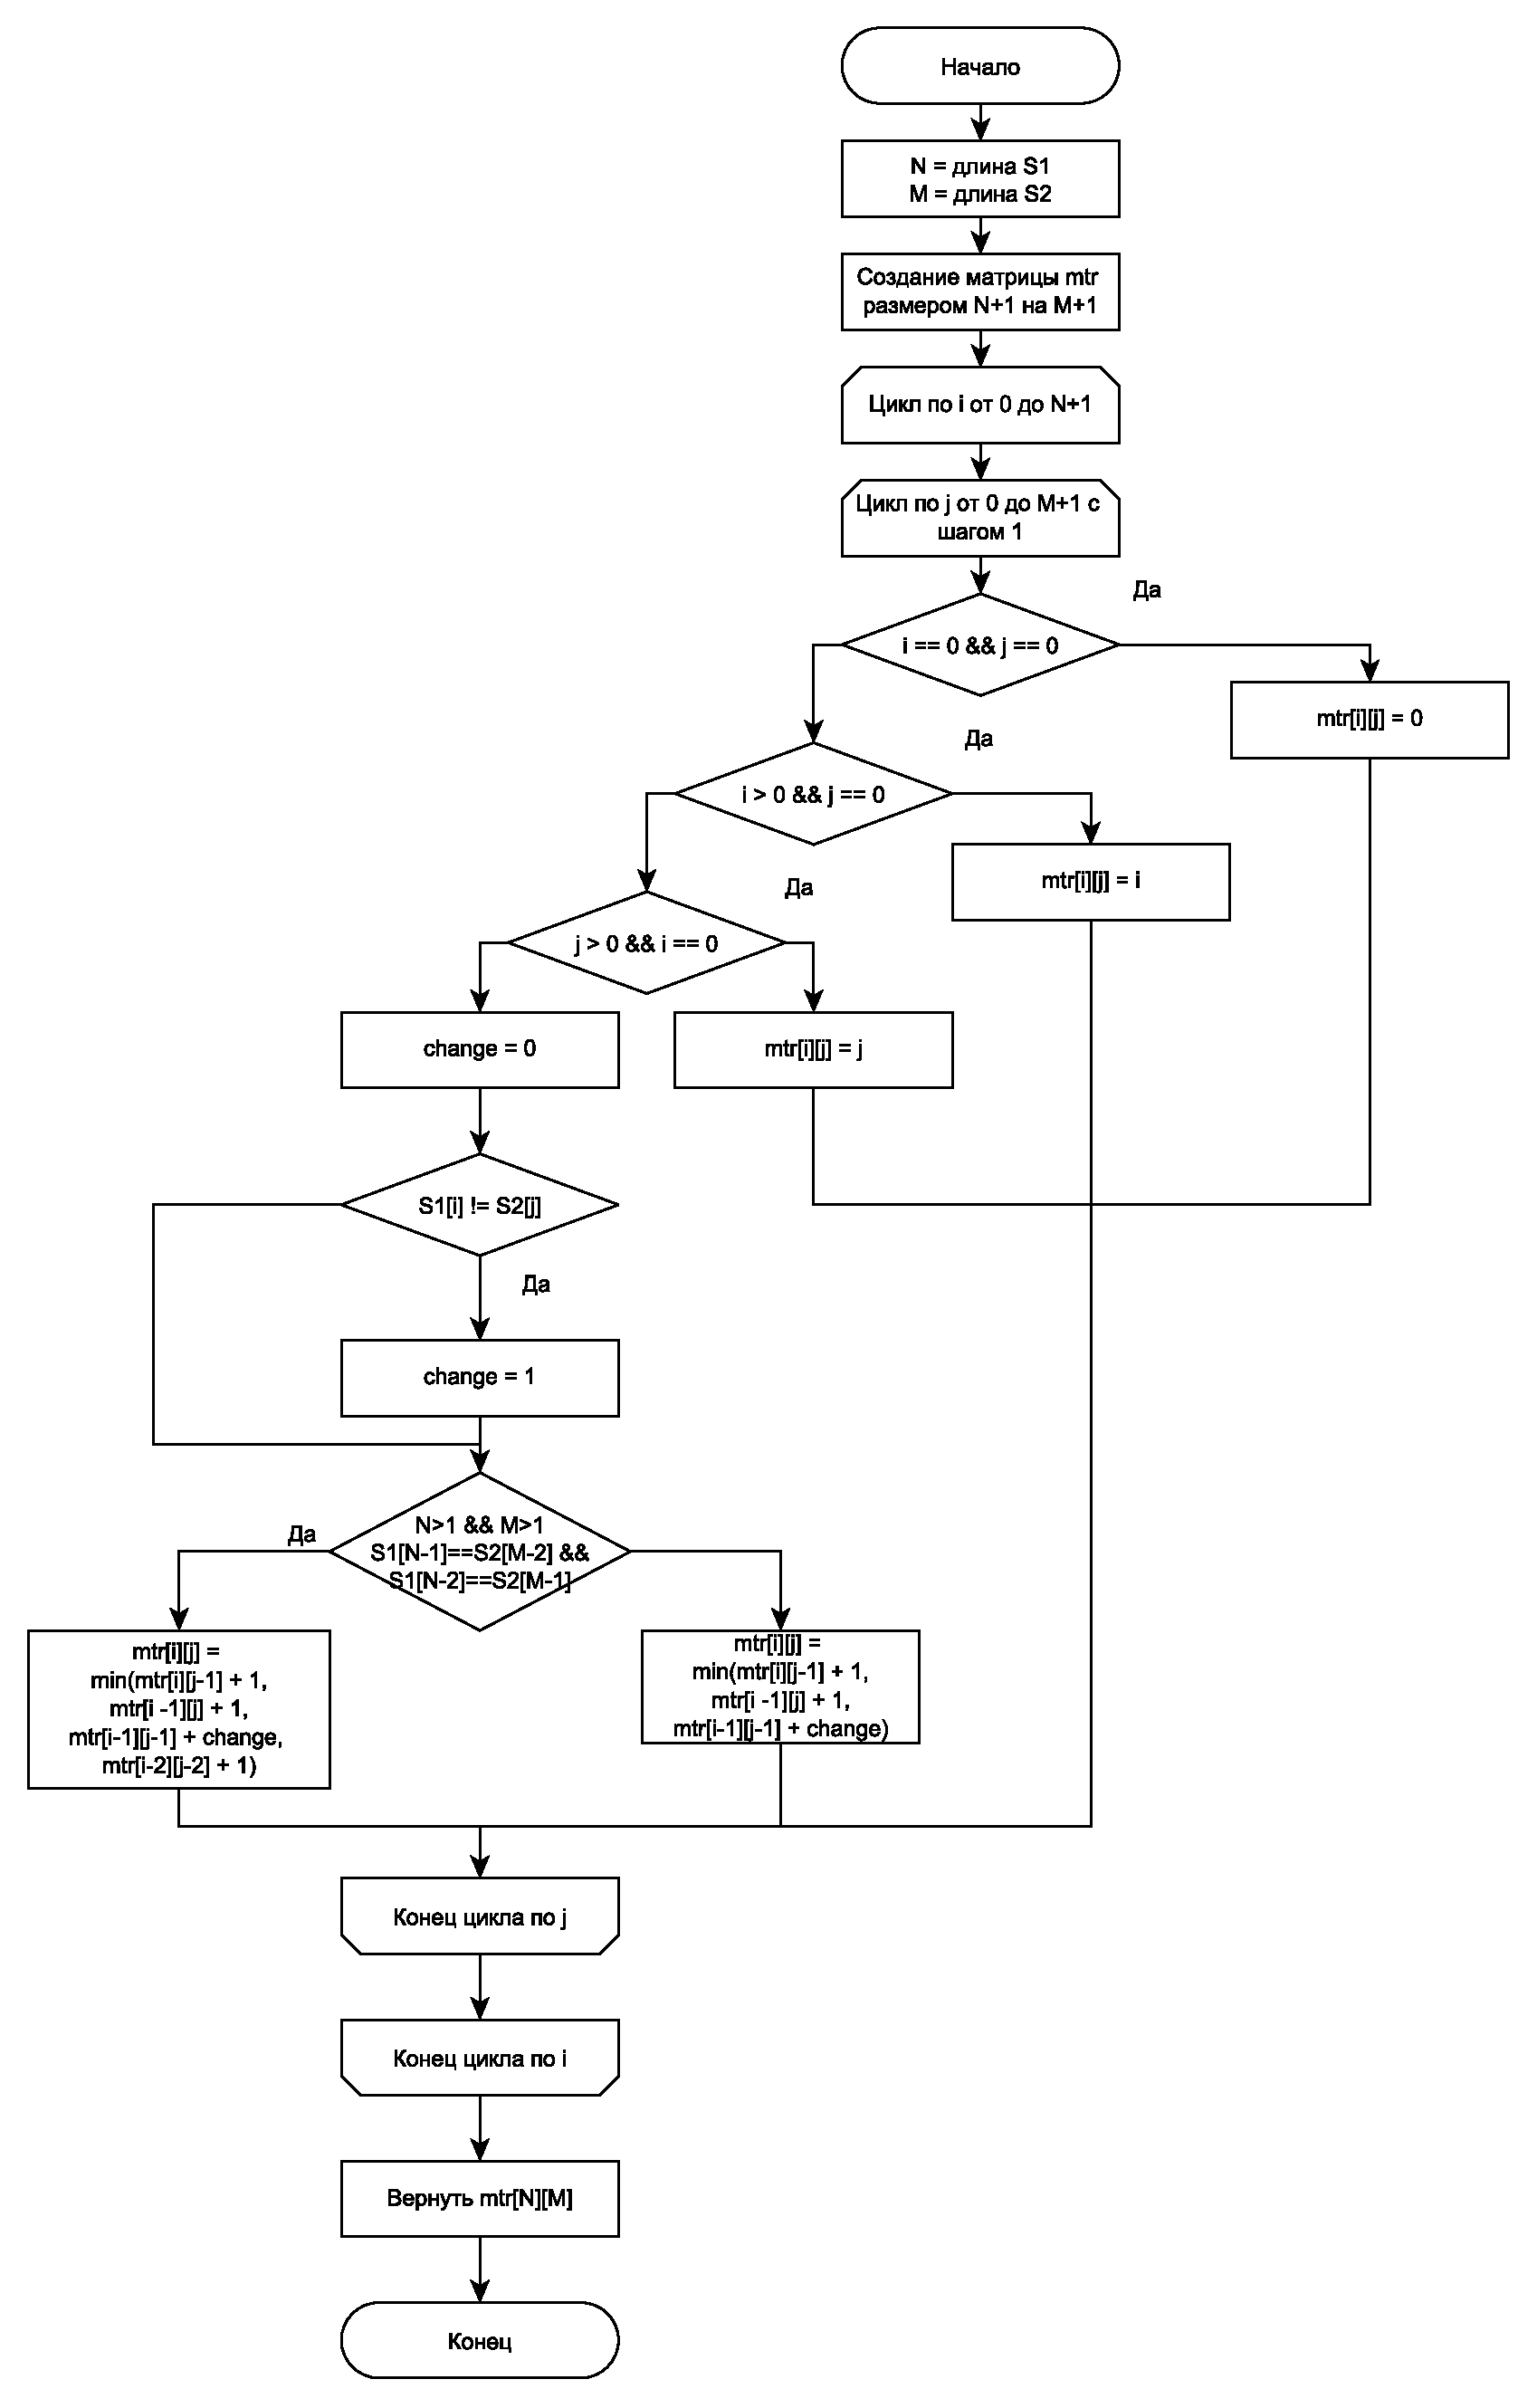
\includegraphics[width=0.8\textwidth]{img/DLiter.pdf} % замените на имя вашего файла
	\caption{Нерекурсивный алгоритм нахождения расстояния Дамерау-Левенштейна}
	\label{fig:DLiter}
\end{figure}

\section{Описание используемых типов и структур данных}

Для реализации алгоритмов, будут использованы следующие типы данных:
\begin{itemize}
	\item  -- для двух строк, поданных на вход;
\end{itemize}